%%%%%%%%%%%%%%%%%%%%%%%%%%%%%%%%%%%%%%%%%%%%%%%%%%%%%%%%%%%%%%%%%%%%%%
% Problem statement
\begin{statement}[
  problempoints=70,
  timelimit=1 sekunda,
  memorylimit=512 MiB,
]{Birmingham}

%\setlength\intextsep{-0.1cm}
%\begin{wrapfigure}[6]{r}{0.22\textwidth}
%\centering
%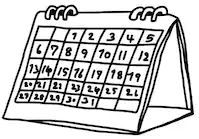
\includegraphics[width=0.22\textwidth]{img/datum.png}
%\end{wrapfigure}

Poznato je da su sve konjičke utrke u Birminghamu namještene danima unaprijed.
Manje je poznato da su određeni ljudi na tajnom sastanku unaprijed dogovorili
tko će biti pobjednik utrke koji već prvi dan nakon sastanka počinju širiti
tu informaciju po gradu. Informacija se širi na sljedeći način.

Prvi dan nakon sastanka, svi ljudi koji znaju informaciju o pobjedniku kažu tu
informaciju svim ljudima do kojih mogu doći u manje ili jednako $K$ koraka.

Drugi dan nakon sastanka, svi ljudi koji znaju informaciju o pobjedniku kažu tu
informaciju svim ljudima do kojih mogu doći u manje ili jednako $2 \cdot K$ koraka.

Općenito, $X$-ti dan nakon sastanka, svi ljudi koji znaju informaciju o
pobjedniku kažu tu informaciju svim ljudima do kojih mogu doći u manje ili
jednako $X \cdot K$ koraka.

Birmingham možemo zamisliti kao graf u kojem čvorovi predstavljaju kuće, a
bridovi dvosmjerne puteljke koji povezuju kuće. Kuće su numerirane prirodnim
brojevima od $1$ do $N$. Kažemo da čovjek može doći do drugog čovjeka u jednom
koraku ako su kuće u kojima žive povezane puteljkom. Od svake kuće je
moguće doći do svake druge kuće u nekom broju koraka.

Vaš je zadatak za svaku kuću ispisati koji će dan nakon sastanka ljudi u toj
kući saznati tko će biti pobjednik utrke.

%%%%%%%%%%%%%%%%%%%%%%%%%%%%%%%%%%%%%%%%%%%%%%%%%%%%%%%%%%%%%%%%%%%%%%
% Input
\subsection*{Ulazni podaci}
U prvom su retku prirodni brojevi $N$, $M$, $Q$ i $K$ $(1 \le N, M, Q, K \le
100\ 000, Q \le N)$, broj kuća u Birminghamu, broj puteljaka koji povezuju kuće, broj
ljudi koji su prisustvovali tajnom sastanku i broj $K$ iz teksta zadatka.

U sljedećem se retku nalazi $Q$ brojeva gdje $i$-ti broj predstavlja oznaku
kuće u kojoj živi $i$-ti čovjek koji je prisustvovao sastanku.

U $i$-tom od sljedećih $M$ redaka nalaze se prirodni brojevi $A_i$ i $B_i$ $(1
\le A_i, B_i \le N, A_i \neq B_i)$, koji nam govore da $i$-ti puteljak
povezuje kuće s oznakama $A_i$ i $B_i$.

%%%%%%%%%%%%%%%%%%%%%%%%%%%%%%%%%%%%%%%%%%%%%%%%%%%%%%%%%%%%%%%%%%%%%%
% Output
\subsection*{Izlazni podaci}
Ispišite $N$ brojeva gdje $i$-ti broj predstavlja koji dan nakon sastanka će
ljudi koji žive u kući s oznakom $i$ saznati tko će pobijediti na utrci. Ako
je čovjek koji živi u kući s oznakom $i$ prisustvovao sastanku, na
odgovarajuće mjesto ispišite $0$.

%%%%%%%%%%%%%%%%%%%%%%%%%%%%%%%%%%%%%%%%%%%%%%%%%%%%%%%%%%%%%%%%%%%%%%
% Scoring
\subsection*{Bodovanje}
U testnim primjerima vrijednima $20$ bodova, vrijedit će $K=1$ i $1 \le N, M
\le 100$.\\
U testnim primjerima vrijednima dodatnih $15$ bodova, vrijedit će $1 \le N, M
\le 100$.

%%%%%%%%%%%%%%%%%%%%%%%%%%%%%%%%%%%%%%%%%%%%%%%%%%%%%%%%%%%%%%%%%%%%%%
% Examples
\subsection*{Probni primjeri}
\begin{tabularx}{\textwidth}{X'X'X}
\sampleinputs{test/birmingham.dummy.in.1}{test/birmingham.dummy.out.1} &
\sampleinputs{test/birmingham.dummy.in.2}{test/birmingham.dummy.out.2} &
\sampleinputs{test/birmingham.dummy.in.3}{test/birmingham.dummy.out.3}
\end{tabularx}

\textbf{Pojašnjenje trećeg probnog primjera:}
TODO SLIKA

Na slici je prikazan graf iz trećeg probnog primjera. Budući da su kuće $1$,
$2$, $3$ i $5$ udaljene za manje ili jednako dva koraka od kuće $6$, onda će
ukućani tih kuća saznati pobjednika prvi dan nakon sastanka. Ukućani kuće $4$
saznat će pobjednika drugi dan nakon sastanka.

%%%%%%%%%%%%%%%%%%%%%%%%%%%%%%%%%%%%%%%%%%%%%%%%%%%%%%%%%%%%%%%%%%%%%%
% We're done
\end{statement}

%%% Local Variables:
%%% mode: latex
%%% mode: flyspell
%%% ispell-local-dictionary: "croatian"
%%% TeX-master: "../hio.tex"
%%% End:
